\documentclass[11pt]{article}
\usepackage[margin=2.5cm]{geometry}
\usepackage{amsmath,amssymb,amsthm,mathtools,booktabs,array}
\usepackage{graphicx}
\usepackage[labelfont=bf,labelsep=space,font=small,justification=raggedright,singlelinecheck=off]{caption}
\renewcommand{\figurename}{Fig.}
\usepackage[hidelinks]{hyperref}
\usepackage[authoryear,round]{natbib}
\newtheorem{proposition}{Proposition}
\newtheorem{lemma}{Lemma}
\newtheorem{theorem}{Theorem}

\begin{document}

\begin{center}
{\large\bfseries What can media-only liver-on-a-chip concentration data identify?\\[2pt]
Structural identifiability, a continuous equivalence family, and a cautionary\\
case study in practical identifiability}\\[6pt]
{\small (adapted for submission to the Journal of Pharmacokinetics and Pharmacodynamics;\\
proofs and the full diagnostic case study in Supplementary Material)}
\end{center}

\begin{abstract}
Contrary to common intuition, no amount of additional media sampling can recover all four kinetic parameters of a liver-on-a-chip clearance model from media concentration data alone: the limitation is structural, not experimental, and it is independent of any specific platform or drug. Liver-on-a-chip systems are used to estimate intrinsic hepatic clearance (CLint) for in vitro-to-in vivo extrapolation. We analyse a minimal two-compartment model (media and cell, linked by distributional clearance CLd and partition coefficient Kp, with non-specific binding kb and metabolism CLint) under media-only sampling, the most common experimental design. Using the Laplace transform of the system, we prove exactly, in closed form, and independently of sampling density or experiment duration, that only three combinations of the four kinetic parameters are structurally identifiable from media concentration data: denser sampling, longer incubations, or better fitting algorithms cannot close this gap. We give the explicit one-parameter family of parameter quadruples -- parametrized by kb -- that all reproduce an identical media concentration curve, up to numerical solver precision. Independently measuring kb, for example via a cell-free non-specific-binding control already used on some platforms, collapses this family to a single point and renders the remaining parameters structurally identifiable. We then show, by direct computation, that standard local methods for assessing practical identifiability are themselves unreliable near this degeneracy: a Fisher-information covariance approximation has condition numbers of $10^9$--$10^{17}$ and disagrees with a pseudoinverse by up to three orders of magnitude on identical data, and a single-start profile likelihood is contaminated by optimizer non-convergence. Multi-start profile likelihood gives a stable result, and that result is sobering: even with kb and evaporation fixed at their true values, CLint remains weakly constrained by realistic sampling designs. Structural identifiability is therefore necessary but not sufficient for practical estimability, and we propose a minimum reporting standard for liver-chip pharmacokinetic studies that would let readers assess both.
\end{abstract}

\noindent\textbf{Keywords:} liver-on-a-chip; structural identifiability; practical identifiability; microphysiological systems; in vitro-in vivo extrapolation; profile likelihood

\section*{Introduction}

Contrary to common intuition, no amount of additional media sampling can recover all four kinetic parameters governing a liver-on-a-chip clearance experiment from media concentration data alone. This is not a limitation of any specific platform, drug, or experimental budget: for the minimal mechanistic structure common to liver-chip clearance analyses, media-only sampling imposes a fundamental information bottleneck that denser sampling, longer incubations, and better fitting algorithms cannot overcome. This paper proves that claim exactly, in closed form, constructs the complete set of parameter combinations it leaves indistinguishable, and then shows that removing this specific bottleneck is still not enough: even once it is removed, the resulting clearance estimate can remain poorly constrained by realistic data, for reasons that have nothing to do with the degeneracy just resolved.

In vitro-to-in vivo extrapolation (IVIVE) of hepatic clearance from conventional assays (microsomes, suspension or plated hepatocytes) systematically underpredicts human pharmacokinetics, by 5- to 10-fold on average across compounds and studies \citep{hallifax2010}. Liver-on-a-chip and related microphysiological systems (MPS) have been proposed as a remedy, offering longer culture viability and more physiologically relevant architecture, and a growing literature applies these platforms to estimate intrinsic clearance (CLint) across several commercial systems, including the CN Bio PhysioMimix \citep{docci2022,tsamandouras2017} and the Javelin liver tissue chip \citep{rajan2023}.

Because liver-chip systems couple medium flow, distribution between medium and cells, metabolism, non-specific binding (NSB) to device materials, and evaporation over multi-day incubations, extracting a clinically interpretable CLint from raw concentration-time data requires more than the single-compartment analysis conventionally applied to microsomal or hepatocyte suspension assays. Several groups have applied formal identifiability analysis to specific configurations. Docci et al.\ \citep{docci2022} performed a priori structural identifiability, via the software DAISY, for three candidate models of their system. Milani et al.\ \citep{milani2022} assessed structural and practical identifiability alongside global sensitivity analysis for a mycophenolate mofetil gut-liver MPS, and Milani et al.\ \citep{milani2024} extended this into a general a priori experimental-design tutorial for organ-on-a-chip systems, demonstrated on midazolam in a gut-liver device, explicitly noting that structural identifiability depends on the specific model structure, dosing, and sampled compartments, and does not guarantee precise practical estimation. Separately, a three-compartment digital-twin approach (DigiLoCS) has been fitted retrospectively to 32 compounds across five published in vitro liver systems, substantially reducing both the bias and the variance of predicted human clearance relative to a conventional depletion analysis \citep{aravindakshan2025}.

Each of these analyses asks whether a specific model, for a specific drug and configuration, is identifiable. None asks the platform-independent question this paper answers: for the minimal mechanistic structure common to liver-chip clearance analyses -- a media compartment exchanging drug with a cell compartment, with first-order NSB and metabolism confined to the cells -- exactly what can the measured media concentration-time curve determine, under the sampling design (media-only, serial) that the overwhelming majority of published studies use \citep{docci2022,rajan2023}, \emph{regardless of which platform or drug generated the data}? That distinction matters: a result proved for one model, one drug, and one device tells a reader whether that experiment was sound; a result proved for the minimal model class itself tells every liver-chip study sharing that structure what it can and cannot claim, before a single data point is collected. And once the answer to that question is known, does resolving it in principle guarantee that the parameters can actually be estimated from realistic, finite, noisy data?

This paper answers both questions. First, using the Laplace transform of the two-compartment system, we prove -- exactly, in closed form, and independently of sampling density, experiment duration, drug identity, or platform -- that media-only sampling recovers only three combinations of the four kinetic parameters (distributional clearance CLd, partition coefficient Kp, intrinsic clearance CLint, and non-specific binding rate kb). We do not stop at showing the fourth combination is unrecoverable: we construct the explicit continuous family of parameter quadruples that are indistinguishable from media data alone, giving any reader a direct, checkable description of the ambiguity rather than an existence statement. We show that independently measuring kb -- for example via a cell-free NSB control, a practice already used on some platforms -- collapses this family to a single point. Second, we test whether resolving this structural degeneracy is sufficient for the parameters to be practically estimable. In doing so we encountered, and report directly, a further finding: standard local methods for quantifying practical identifiability (Fisher-information-based covariance approximations and single-start profile likelihood) are themselves numerically unreliable near this type of structural degeneracy, and only a more computationally demanding multi-start profile likelihood gives a trustworthy answer. That answer shows that fixing kb and evaporation at their true values does not, by itself, sharpen the practical identifiability of CLint under realistic sampling designs. We close by proposing a minimum set of reporting items that would let a reader independently assess both the structural and practical identifiability of a published liver-chip CLint estimate.

\section*{Theoretical}

\subsection*{Model}

We consider the minimal mechanistic structure common to liver-chip clearance analyses: a media compartment (concentration $C_m$, volume $V_m$) exchanging drug with a lumped cell-associated compartment (concentration $C_c$, volume $V_c$), linked by a distributional clearance $CL_d$ and a cell:media partition coefficient $K_p$, with first-order non-specific binding (NSB) loss from media at rate $k_b$, and metabolism (intrinsic clearance $CL_{int}$) confined to the cell compartment:
\begin{align}
\frac{dC_m}{dt} &= -\frac{CL_d}{V_m}C_m + \frac{CL_d}{K_p V_m}C_c - k_b C_m, \label{eq:cm}\\
\frac{dC_c}{dt} &= \frac{CL_d}{V_c}C_m - \left(\frac{CL_d}{K_p V_c} + \frac{CL_{int}}{V_c}\right)C_c. \label{eq:cc}
\end{align}
In matrix form $\dot{\mathbf{x}} = A\mathbf{x}$ with $\mathbf{x} = [C_m, C_c]^T$,
\[
A = \begin{pmatrix} a_{11} & a_{12} \\ a_{21} & a_{22} \end{pmatrix}, \quad
a_{11} = -\left(\frac{CL_d}{V_m} + k_b\right),\ a_{12} = \frac{CL_d}{K_p V_m},\ a_{21} = \frac{CL_d}{V_c},\ a_{22} = -\left(\frac{CL_d}{K_p V_c} + \frac{CL_{int}}{V_c}\right).
\]
This is structurally the same class of model used by Docci et al.\ \citep{docci2022}, the DigiLoCS digital twin \citep{aravindakshan2025}, and Milani et al.'s gut-liver OoC framework \citep{milani2022,milani2024}, restricted here to a single tissue compartment and constant volume; evaporation is addressed separately below. $V_m$ and $V_c$ are fixed, known hardware parameters; $CL_d$, $K_p$, $CL_{int}$, $k_b$ are the four unknown kinetic parameters.

This reduction is deliberate rather than a simplifying convenience. Every richer liver-chip model in current use --- additional compartments, reversible rather than first-order NSB, intracellular sub-structure --- contains this two-compartment system as the core process linking an observed media signal to an unobserved intracellular metabolic rate. An identifiability obstruction present in this minimal core is therefore a necessary feature, not an artifact of simplification: a richer model can only fail to inherit it by adding structure that specifically breaks the degeneracy (for example, an additional observed compartment), not by adding structure that leaves the media-to-cell link otherwise intact. The minimal model is accordingly the right place to prove an exact, general result; we return to what is and is not known about richer models directly in the Discussion.

\subsection*{Structural identifiability of media-only sampling}

The overwhelming majority of published liver-chip PK studies sample only the media compartment serially, reserving any cell-associated (lysate) measurement for a single endpoint, if at all \citep{docci2022,rajan2023}. Taking the Laplace transform of Eqs.~\eqref{eq:cm}--\eqref{eq:cc} with an impulse-type initial condition (dose in media only, $C_m(0)=C_0$, $C_c(0)=0$) and observing $y(t)=C_m(t)$, the transfer function is
\begin{equation}
\frac{Y(s)}{C_0} = \frac{s - a_{22}}{s^2 - (a_{11}+a_{22})s + (a_{11}a_{22} - a_{12}a_{21})}. \label{eq:transferfn}
\end{equation}
Only three quantities are recoverable from concentration-time data of arbitrary duration and density, however dense or extended: $a_{11}$, $a_{22}$, and the product $a_{12}a_{21} = CL_d^2/(K_p V_m V_c) \equiv P$. With $V_m$ and $V_c$ known, this gives
\begin{equation}
a_{11} = -\left(\frac{CL_d}{V_m}+k_b\right), \qquad a_{22} = -\left(\frac{CL_d}{K_p V_c}+\frac{CL_{int}}{V_c}\right), \qquad P = \frac{CL_d^2}{K_p V_m V_c}, \label{eq:threeeqns}
\end{equation}
\textbf{three equations in the four unknowns} $CL_d$, $K_p$, $CL_{int}$, $k_b$: the model is structurally unidentifiable from media-only sampling, by exactly one degree of freedom. This conclusion is exact, holds in closed form, and depends on nothing but the structure of Eqs.~\eqref{eq:cm}--\eqref{eq:cc}: it is unaffected by how many samples are taken, how long the incubation runs, which drug is studied, or which commercial platform generated the data. No improvement in sampling density, experiment duration, or fitting procedure can recover the missing degree of freedom, because it is not missing from the data by accident --- it is absent from what the model structure makes observable in the first place.

\subsubsection*{The continuous equivalence family}

Equation~\eqref{eq:threeeqns} can be solved explicitly for $CL_d$, $K_p$, $CL_{int}$ in terms of a free parameter $k_b$:
\begin{equation}
CL_d(k_b) = V_m(-a_{11}-k_b), \qquad K_p(k_b) = \frac{CL_d(k_b)^2}{P\,V_m V_c}, \qquad CL_{int}(k_b) = -a_{22}V_c - \frac{CL_d(k_b)}{K_p(k_b)}. \label{eq:family}
\end{equation}
Choosing any admissible $k_b$ (yielding positive $CL_d$, $K_p$, $CL_{int}$) defines a corresponding parameter quadruple $(CL_d, K_p, CL_{int}, k_b)$ consistent with the same $(a_{11}, a_{22}, P)$, and therefore the same media concentration trajectory $C_m(t)$, exactly. Figure~\ref{fig:degeneracy}a illustrates this numerically: two parameter quadruples differing by up to 4-fold in each parameter --- $(CL_d, K_p, CL_{int}, k_b) = (8.0, 5.0, 4.5, 0.0008)$ and $(4.48, 1.57, 3.24, 0.003)$ --- produce media concentration trajectories that are visually indistinguishable over a simulated 33-hour incubation. Figure~\ref{fig:degeneracy}b shows the relative difference between the two trajectories directly: it remains below $4\times10^{-7}$ throughout, consistent with the two parameter sets being related by Eq.~\eqref{eq:family} and differing only by the numerical tolerance of the ODE solver, not by any genuine difference in the predicted observable.

\subsubsection*{Resolution via independent measurement of $k_b$}

Independent characterization of $k_b$ --- for example via a cell-free NSB control, already run by Docci et al.\ and Rajan et al.\ \citep{docci2022,rajan2023} --- collapses the family in Eq.~\eqref{eq:family} to a single point, making $CL_d$, $K_p$, and $CL_{int}$ structurally identifiable via the same three relations. This is not the only route: intracellular sampling, or independently fixing $K_p$ or $CL_d$, would work equally well \citep{milani2024}. The result applies to the stated first-order NSB representation; real device adsorption can be reversible and compound-class-dependent (Rajan et al.\ found $>$85\% recovery for 17 of 21 compounds, but appreciably lower recovery for some lipophilic acidic drugs \citep{rajan2023}), so a cell-free recovery experiment characterizes $k_b$ for that representation, not necessarily every loss mechanism at play. Evaporation is more tractable: because it manifests as a measurable $V_m(t)$, it can in principle be supplied to the model as a known input rather than estimated jointly, provided the volume trajectory and any sampling withdrawals are adequately characterized.

At this point it is tempting to conclude that measuring $k_b$ settles the matter: the structural degeneracy is resolved, and $CL_d$, $K_p$, $CL_{int}$ become uniquely determined. This is correct as a statement about noise-free data of infinite precision. It is not, by itself, a statement about what a real experiment with finite samples and realistic noise can estimate. Structural identifiability guarantees that a unique answer exists; it says nothing about how sharply that answer is pinned down once noise is introduced. We return to this distinction directly, with a worked demonstration, in the Results.

\subsection*{Exact bias limits of conventional single-compartment analysis}

Define the conventional apparent clearance as $CL_{naive} = V_m k_{dep}$, where $k_{dep}$ is the monoexponential media-depletion rate constant an analyst would fit assuming a single well-mixed compartment at constant $V_m$ (the eigenvalue of $A$ with smaller magnitude). Two asymptotic regimes admit exact closed-form limits.

\textbf{Fast-distribution limit} ($CL_d/CL_{int}\to\infty$): as $CL_d\to\infty$ with the other parameters fixed,
\begin{equation}
CL_{naive} \to \frac{V_m(K_p CL_{int} + k_b V_m)}{V_m + K_p V_c}. \label{eq:fastdist}
\end{equation}

\textbf{Fast-metabolism limit} ($CL_{int}/CL_d\to\infty$): as $CL_{int}\to\infty$, the cell compartment behaves as an absorbing sink and
\begin{equation}
CL_{naive} \to CL_d + k_b V_m, \label{eq:fastmetab}
\end{equation}
independent of $CL_{int}$.

Nondimensionalizing with $\tau = (CL_d/V_m)t$, $x = C_m/C_m(0)$, $y = C_c/(K_p C_m(0))$ reduces Eqs.~\eqref{eq:cm}--\eqref{eq:cc} to
\begin{equation}
\frac{dx}{d\tau} = -(1+\beta)x + y, \qquad \frac{dy}{d\tau} = \frac{1}{r}\left[x - (1+\mu)y\right], \label{eq:nondim}
\end{equation}
where $r = K_p V_c/V_m$, $\beta = k_b V_m/CL_d$, and $\mu = K_p CL_{int}/CL_d$. The dimensionless concentration dynamics $x(\tau)$ are governed by exactly these three groups: nominally different platforms produce identical trajectories whenever $r$, $\beta$, and $\mu$ coincide, regardless of absolute volumes or cell numbers. The bias ratio $CL_{naive}/CL_{int}$ depends additionally on $K_p$ directly, since it compares apparent clearance against $CL_{int}$ rather than comparing dynamics alone: in these terms, the fast-distribution limit is $CL_{naive}/CL_{int} \to [K_p/(1+r)](1+\beta/\mu)$, reducing to $K_p/(1+r)$ when NSB is negligible relative to metabolism ($\beta\ll\mu$); the fast-metabolism limit is $CL_{naive}/CL_{int} \to (K_p/\mu)(1+\beta)$. Thus, as $CL_{int}/CL_d\to\infty$, the apparent-to-intrinsic clearance ratio tends to zero, producing arbitrarily severe underestimation; in the fast-distribution limit, the bias direction instead depends on $K_p$, $r$, and the relative NSB contribution.

\begin{table}[t]
\centering
\caption{Minimum reporting checklist for liver-chip pharmacokinetic studies intended to support IVIVE}
\label{tab:checklist}
\begin{tabular}{@{}cp{11cm}@{}}
\toprule
\# & Item \\
\midrule
1 & Compartment volumes and sampling/replacement volumes \\
2 & Cell number or measured functional cell mass \\
3 & Flow/recirculation rate and geometry \\
4 & Evaporation trajectory \\
5 & Compound-specific cell-free recovery/NSB data \\
6 & Raw concentration-time data with below-LOQ values identified \\
7 & Actual sampling times and analytical LOQ \\
8 & Model equations, parameter definitions, units, externally fixed parameters \\
\midrule
9 & \textit{(recommended)} Structural identifiability assessment for the specified observation scheme \\
10 & \textit{(recommended)} Practical-identifiability/uncertainty analysis using a method appropriate near any known structural degeneracy, not point estimates alone \\
\bottomrule
\end{tabular}
\end{table}

\section*{Methods}

\paragraph{Platform and ground-truth parameters.} Illustrative calculations use the CN Bio PhysioMimix hardware parameters reported by Docci et al.\ \citep{docci2022}: media volume $V_m = 1600\ \mu$L, cell-compartment volume $V_c = 3\ \mu$L (a nominal small volume, not independently reported), $3\times10^5$ cells. Ground-truth kinetic parameters ($CL_d = 8.0\ \mu$L/min, $K_p = 5.0$, $k_b = 0.0008$ min$^{-1}$) are illustrative, chosen to be broadly consistent with the orders of magnitude reported for liver-chip systems, and are not fitted to any specific compound. Two $CL_{int}$ levels were used: a ``low'' level (total $CL_{int} = 0.3\ \mu$L/min, corresponding to $1.0\ \mu$L/min per $10^6$ cells) and a ``high'' level (total $CL_{int} = 15.0\ \mu$L/min, corresponding to $50.0\ \mu$L/min per $10^6$ cells), spanning part of the $\sim$800-fold range of intrinsic clearances reported across compounds by Rajan et al.\ \citep{rajan2023}.

\paragraph{Structural identifiability and the equivalence family.} Equation~\eqref{eq:threeeqns} was solved symbolically (SymPy) for $(CL_d, K_p, CL_{int})$ in terms of a free $k_b$, yielding Eq.~\eqref{eq:family}. This closed-form family was verified numerically by substituting two specific parameter quadruples differing up to 4-fold --- the ground-truth quadruple and a second quadruple obtained from Eq.~\eqref{eq:family} at a different $k_b$ --- into the full nonlinear ODE system (Eqs.~\eqref{eq:cm}--\eqref{eq:cc}, constant volume, $e=0$) and numerically integrating both (\texttt{scipy.integrate.solve\_ivp}, method LSODA, relative tolerance $10^{-9}$, absolute tolerance $10^{-12}$) over a simulated 2000-minute incubation. The two resulting $C_m(t)$ trajectories were compared directly (Fig.~\ref{fig:degeneracy}).

\paragraph{Exact asymptotic limits.} Equations~\eqref{eq:fastdist}--\eqref{eq:fastmetab} were derived analytically from the eigenvalues of $A$ in the limits $CL_d\to\infty$ and $CL_{int}\to\infty$ respectively, and confirmed by direct numerical eigenvalue evaluation across $CL_d \in \{8, 80, \dots, 8\times10^{12}\}\ \mu$L/min and $CL_{int} \in \{4.5, 45, \dots, 4.5\times10^{10}\}\ \mu$L/min (other parameters fixed at ground truth), matching the closed-form limits to 5 significant figures before floating-point noise appeared. The nondimensionalization (Eq.~\eqref{eq:nondim}) was derived by substitution and confirmed symbolically.

\paragraph{Synthetic data generation.} For a given platform, drug, dose, and sampling schedule, noise-free $C_m(t)$ was simulated by numerical integration as above. Proportional Gaussian noise (coefficient of variation 15\%, representative of LC-MS/MS assay variability) was added to generate synthetic ``observed'' data, with a fixed random seed for reproducibility. Sparse designs used 5 samples and dense designs used 12 samples, log-spaced or evenly spaced across an incubation window chosen adaptively per scenario (shorter for high-clearance compounds, consistent with the use of shorter incubation windows for high-clearance compounds and longer windows for low-clearance compounds in practice \citep{rajan2023}).

\paragraph{Mechanistic model fitting.} All five kinetic/loss parameters ($CL_{int}$, $CL_d$, $K_p$, $k_b$, evaporation rate $e$) were fitted jointly to synthetic data by nonlinear least squares on log-transformed residuals (\texttt{scipy.optimize.least\_squares}, trust-region-reflective algorithm, bounded), starting from perturbed values near the ground truth as a literature-informed analyst's initial guess would be.

\paragraph{Practical identifiability: Fisher information.} At the fitted optimum, the Gauss-Newton Fisher Information Matrix $J^TJ$ was computed from the Jacobian of the residuals. The relative standard error of $CL_{int}$ was computed two ways: via plain matrix inversion (\texttt{numpy.linalg.inv}) and via a truncated-SVD pseudoinverse (\texttt{numpy.linalg.pinv}, \texttt{rcond}=$10^{-10}$), for two representative scenarios (low- and high-$CL_{int}$, dense sampling). The condition number of $J^TJ$ was computed for both scenarios (Fig.~\ref{fig:fim}).

\paragraph{Practical identifiability: profile likelihood.} For the low-$CL_{int}$, sparse-sampling scenario, a profile likelihood for $CL_{int}$ was computed by fixing $CL_{int}$ at a grid of values relative to its fitted value (ratios 0.2 to 19.2), re-optimizing the remaining free parameters at each grid point from a single fixed starting point (\emph{single-start}), and recording the resulting sum of squared residuals (SSE) relative to the unconstrained optimum. This was repeated with 6 random restarts per grid point, retaining the best (lowest-SSE) fit at each point (\emph{multi-start}), for three scenarios: sparse sampling with $k_b$ and evaporation $e$ unknown (jointly fitted); sparse sampling with $k_b$ and $e$ fixed at their true values; and dense sampling with $k_b$ and $e$ fixed. A 95\% confidence region was defined by the $\chi^2_1$ threshold ($\Delta$SSE $\le 3.84\,\sigma^2$, with $\sigma^2$ the residual variance at the optimum) (Fig.~\ref{fig:profile}).

\paragraph{Software and reproducibility.} All calculations were performed in Python 3 (NumPy, SciPy, SymPy, Matplotlib). Code implementing every result in this paper, including the figures, is provided as Supplementary Material and will be deposited in a public repository.

\section*{Results}

\subsection*{A continuous family of indistinguishable parameter sets}

Figure~\ref{fig:degeneracy}a shows two parameter quadruples related by Eq.~\eqref{eq:family} --- $(CL_d, K_p, CL_{int}, k_b) = (8.0\ \mu\text{L/min}, 5.0, 4.5\ \mu\text{L/min}, 0.0008\ \text{min}^{-1})$ and $(4.48\ \mu\text{L/min}, 1.57, 3.24\ \mu\text{L/min}, 0.003\ \text{min}^{-1})$, differing by up to 4-fold in each individual parameter --- simulated through the full nonlinear ODE system over a 33-hour incubation. The two resulting media concentration-time curves are visually superimposed throughout. Figure~\ref{fig:degeneracy}b shows the relative difference between the two curves directly: it remains below $3.9\times10^{-7}$ at every time point, consistent with the two trajectories being analytically identical and differing only at the level of numerical solver tolerance. This confirms, for a specific worked example, that the continuous equivalence family derived in Eq.~\eqref{eq:family} is not merely a formal algebraic statement but corresponds to a genuine, exact observational indistinguishability.

\begin{figure}[t]
\centering
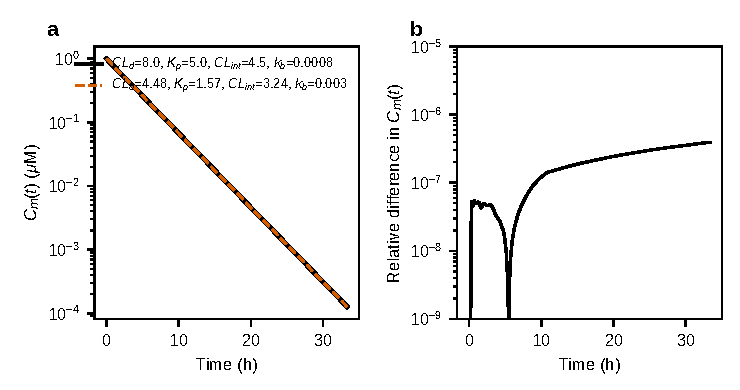
\includegraphics[width=0.75\textwidth]{figures/Fig2}
\caption{A continuous family of parameter quadruples produces identical media concentration-time data. \textbf{(a)} Media concentration $C_m(t)$ simulated from two parameter quadruples related by Eq.~\eqref{eq:family} (CN Bio hardware, constant-volume reduction). \textbf{(b)} Relative difference between the two trajectories in panel (a), remaining below $4\times10^{-7}$ throughout, consistent with numerical solver precision rather than a genuine difference in the predicted observable.}
\label{fig:degeneracy}
\end{figure}

\subsection*{Local uncertainty diagnostics are numerically unreliable near the degeneracy}

For the low-$CL_{int}$, dense-sampling scenario, the Gauss-Newton Fisher Information Matrix $J^TJ$ at the fitted optimum had a condition number of $1.38\times10^{17}$ (Fig.~\ref{fig:fim}a) --- at or beyond the limit of double-precision numerical reliability. For the high-$CL_{int}$, dense-sampling scenario, the condition number was $1.45\times10^{12}$, also indicating a numerically near-singular matrix. Correspondingly, the relative standard error of $CL_{int}$ computed via plain matrix inversion disagreed sharply with the same quantity computed via a truncated-SVD pseudoinverse on identical data: $1.40\times10^3$ (plain) versus $6.9$ (pseudoinverse) for the low-$CL_{int}$ scenario, and $2.4$ versus $0.19$ for the high-$CL_{int}$ scenario (Fig.~\ref{fig:fim}b) --- disagreements of two to three orders of magnitude from the choice of inversion algorithm alone, on the same fitted model and the same data.

\begin{figure}[t]
\centering
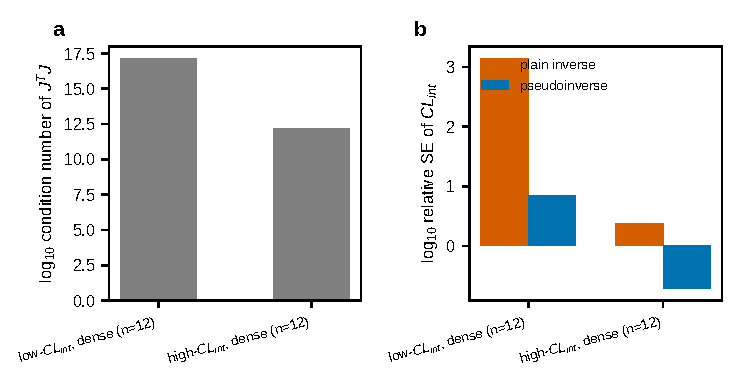
\includegraphics[width=0.75\textwidth]{figures/Fig3}
\caption{Fisher-information-based practical identifiability diagnostics are numerically unstable near the structural degeneracy. \textbf{(a)} Condition number of the Gauss-Newton Fisher Information Matrix $J^TJ$ at the fitted optimum, for two representative scenarios (dense sampling, $n=12$). \textbf{(b)} Relative standard error of $CL_{int}$ computed via plain matrix inversion versus a truncated-SVD pseudoinverse, on identical fitted data.}
\label{fig:fim}
\end{figure}

\subsection*{Single-start profile likelihood is contaminated by optimizer non-convergence}

A profile likelihood for $CL_{int}$, computed with a single optimizer start per grid point (low-$CL_{int}$, sparse sampling, $k_b$ and $e$ jointly fitted), was non-monotonic and erratic (Fig.~\ref{fig:profile}a): $\Delta$SSE remained near zero at most grid points but spiked to 0.34 at a ratio of 4.8 before falling again at larger ratios. This pattern --- a profile that is not unimodal and does not increase monotonically away from the optimum --- is inconsistent with a genuine likelihood profile and is instead diagnostic of the optimizer failing to locate the true conditional optimum at some grid points when started from a single, non-adaptive initial guess.

\subsection*{Multi-start profile likelihood: structural identifiability does not guarantee practical estimability}

Repeating the profile likelihood computation with 6 random restarts per grid point, retaining the best fit at each point, gave materially more stable profiles (Fig.~\ref{fig:profile}b). Three findings follow. First, with $k_b$ and $e$ unknown (jointly fitted) and sparse sampling, $\Delta$SSE remained near zero (all 7 scanned points inside the 95\% confidence region) across the full scanned range of $CL_{int}$ ratios (0.3$\times$ to 3.0$\times$ the true value): $CL_{int}$ is not practically constrained by this design, consistent with the structural degeneracy identified in Eq.~\eqref{eq:family}. Second, fixing $k_b$ and $e$ at their true values --- which Eq.~\eqref{eq:family} shows should render the model structurally identifiable --- did \emph{not}, in this regime, sharpen the practical identifiability of $CL_{int}$: all 7 scanned points remained inside the 95\% confidence region for sparse sampling with $k_b$, $e$ known. Third, this remained true even under dense sampling ($n=12$) with $k_b$ and $e$ known: again all 7 scanned points were inside the 95\% confidence region. In other words, removing the exact structural degeneracy by independently fixing $k_b$ and $e$ did not, by itself, translate into a practically well-constrained estimate of $CL_{int}$ in this low-clearance regime, regardless of sampling density.

\begin{figure}[t]
\centering
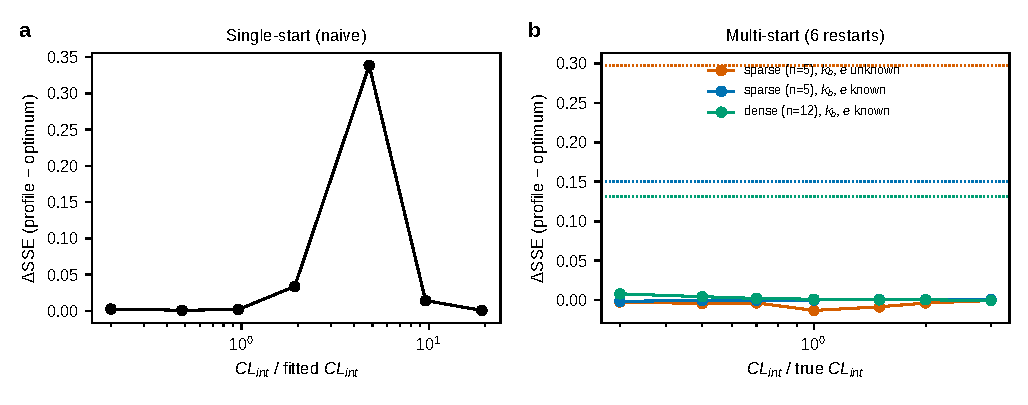
\includegraphics[width=\textwidth]{figures/Fig4}
\caption{Single-start profile likelihood is unreliable; multi-start profile likelihood reveals that resolving the structural degeneracy does not guarantee practical identifiability. \textbf{(a)} Profile likelihood for $CL_{int}$ with a single optimizer start per grid point (low-$CL_{int}$, sparse sampling, $k_b$ and $e$ jointly fitted), showing a non-monotonic, erratic profile diagnostic of optimizer non-convergence. \textbf{(b)} Profile likelihoods with 6 random restarts per grid point, for three scenarios; dotted horizontal lines mark the 95\% ($\chi^2_1$) confidence threshold for each scenario (color-matched). All three profiles remain within their respective 95\% thresholds across the full scanned range.}
\label{fig:profile}
\end{figure}

\subsection*{Summary figure}

Figure~\ref{fig:schematic} summarizes the overall argument: media-only concentration data determine three combinations of the four kinetic parameters, not the parameters themselves (panel A); the resulting one-parameter family of indistinguishable solutions collapses to a point once $k_b$ is independently measured (panel B); and structural identifiability, so achieved, is necessary but not sufficient for practical estimability, which must be assessed separately and explicitly (panel C), as demonstrated directly in Fig.~\ref{fig:profile}.

\begin{figure}[t]
\centering
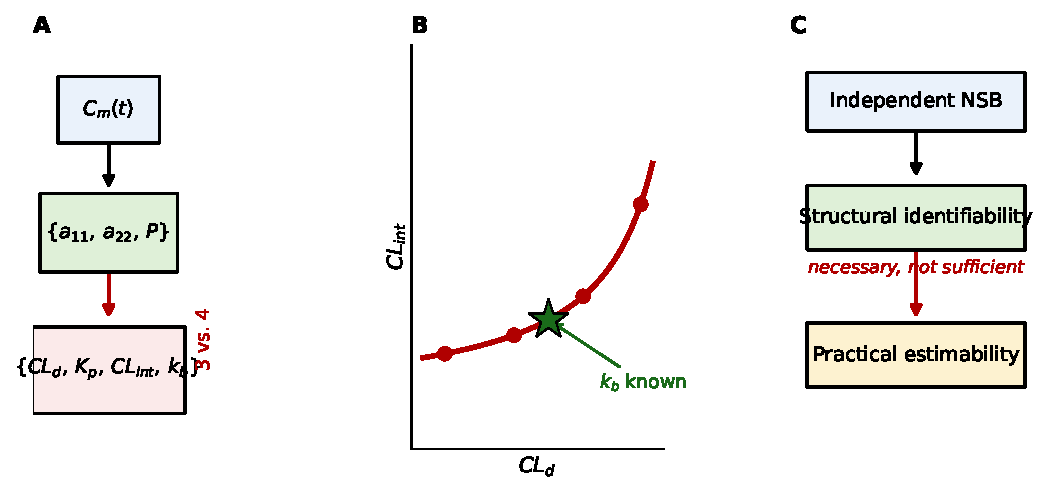
\includegraphics[width=\textwidth]{figures/Fig1}
\caption{Schematic summary. \textbf{(A)} Information bottleneck: media concentration data $C_m(t)$ determine only three combinations $\{a_{11}, a_{22}, P\}$ of the four mechanistic parameters $\{CL_d, K_p, CL_{int}, k_b\}$. \textbf{(B)} The resulting continuous equivalence family (schematic), parametrized by $k_b$; independent measurement of $k_b$ selects the true point. \textbf{(C)} Structural identifiability, once achieved, is necessary but not sufficient for practical estimability.}
\label{fig:schematic}
\end{figure}

\section*{Discussion}

\subsection*{What media-only sampling can and cannot tell us}

The central result of this paper is exact and independent of any particular drug or platform: a minimal two-compartment liver-chip model, observed through media-only sampling, is structurally unidentifiable by precisely one degree of freedom, and the entire one-parameter family of equally consistent parameter quadruples can be written in closed form (Eq.~\eqref{eq:family}). This is not a statement about insufficient data density or duration --- the three identifiable combinations $a_{11}$, $a_{22}$, $P$ are exactly what the media concentration-time curve can ever determine, however many samples are taken or however long the incubation runs. The practical corollary is that a cell-free non-specific-binding control, already standard practice on some but not all liver-chip platforms, is not merely good laboratory hygiene: it is a mathematical precondition for the remaining kinetic parameters to be identifiable at all from this type of experiment.

\subsection*{A methodological finding: local diagnostics can mislead near a structural degeneracy}

Beyond the structural result, this work surfaced a second, more general methodological finding that we believe is of independent interest. Near a structural (or near-structural) degeneracy, the standard toolkit for quantifying how well a parameter is constrained by data can itself become unreliable. We observed this directly: a Fisher-information covariance approximation gave condition numbers of $10^{12}$ to $10^{17}$, and switching between a plain matrix inverse and a pseudoinverse on identical fitted data changed the estimated relative standard error of $CL_{int}$ by two to three orders of magnitude. Our first response --- adopting the pseudoinverse as the more numerically stable choice --- turned out to be informative in the wrong direction: a direct profile-likelihood check showed that the pseudoinverse-based estimate was misleadingly optimistic relative to the genuinely flat likelihood surface. A single-start profile likelihood, often treated as the more rigorous alternative to a covariance approximation, was itself unreliable here, producing a non-monotonic profile attributable to the optimizer failing to converge at some grid points. Only a multi-start profile likelihood, which is substantially more computationally expensive, gave a profile we are confident reflects the actual information content of the data. We report this progression explicitly, including the dead ends, because it is a cautionary tale with a clear methodological implication: near a known or suspected structural degeneracy, point estimates and standard practical-identifiability diagnostics should not be trusted without a multi-start or otherwise global check.

\subsection*{Structural identifiability is necessary, not sufficient}

The multi-start profile likelihood result in Fig.~\ref{fig:profile}b is, on its own, a finding that qualifies the paper's main structural message. Resolving the exact structural degeneracy by fixing $k_b$ and evaporation $e$ at their true values is, by Eq.~\eqref{eq:family}, sufficient to make the model structurally identifiable --- a unique solution exists in the noise-free, infinite-data limit. It did not, in the regime we examined (low $CL_{int}$ relative to $CL_d$), translate into a practically well-constrained estimate of $CL_{int}$ under either sparse or dense realistic sampling. This is consistent with the broader point made by Milani et al.\ \citep{milani2024} that structural identifiability does not guarantee precise practical estimation, and it sharpens that point by showing a concrete case in which the gap persists even after the specific structural obstruction (the $k_b$-parametrized equivalence family) has been removed. We did not characterize how this result depends on the regime (the ratio of $CL_{int}$ to $CL_d$, captured by the dimensionless group $\mu$ in Eq.~\eqref{eq:nondim}); this is a natural direction for further work.

\subsection*{Relationship to prior identifiability work on organ-on-a-chip systems}

Docci et al.\ \citep{docci2022} performed a priori structural identifiability analysis, via DAISY, for three candidate models of their specific PhysioMimix configuration. Milani et al.\ \citep{milani2022} assessed structural and practical identifiability for a mycophenolate mofetil gut-liver system, and Milani et al.\ \citep{milani2024} generalized this into an a priori experimental-design workflow (structural identifiability, global dynamic sensitivity analysis, and simulation-based verification) demonstrated on midazolam. The distinction between that body of work and this paper is categorical, not incremental: each of those analyses asks whether \emph{one} model is identifiable, for \emph{one} drug, on \emph{one} device, and answers that question by running the check on that specific case. This paper instead proves a theorem about the minimal model class itself --- exact, closed-form, and true for every drug and every platform sharing that structure, before any specific experiment is designed or any specific DAISY check is run. A reader of Docci et al.\ or Milani et al.\ learns whether \emph{that} experiment was identifiable; a reader of this paper learns what any media-only liver-chip experiment of this structure can and cannot claim, in advance. Our contribution is complementary to, not a replacement for, model-specific checks: it tells a reader what to expect before running one, together with a direct demonstration that the practical-identifiability side of any such workflow requires a global (multi-start or equivalent) method to be trusted. The three-compartment DigiLoCS digital twin \citep{aravindakshan2025} adds a further compartment (media, interstitium, and intracellular space) to the structure considered here; whether an analogous equivalence family exists in that richer model, and whether it is removed by the same NSB-control strategy, is an open question raised directly by our result.

\subsection*{Toward a minimum reporting standard}

Existing microphysiological system quality-management recommendations \citep{pamies2024} address biological reproducibility, not what a study must report for independent identifiability assessment. Table~\ref{tab:checklist} sets out items we believe a liver-chip PK study should report if its CLint estimate is intended to support IVIVE: the first eight are items that should simply be reported; the final two --- a structural identifiability assessment for the specific observation scheme used, and a practical-identifiability or uncertainty analysis robust to the kind of degeneracy demonstrated here --- are analyses we recommend performing, not merely data to disclose.

\subsection*{Limitations}

$K_p$, $CL_d$, and the specific numerical values used in our worked examples are illustrative and not fitted to any specific compound; the qualitative structural and methodological results do not depend on these choices, but their magnitudes do. The closed-form structural result (Eq.~\eqref{eq:family}) is exact for the constant-volume reduction of the model; we did not perform a DAISY-based or equivalent structural analysis of the complete five-parameter, time-varying-volume model that includes evaporation as a jointly fitted (rather than externally measured) quantity. We examined the practical-identifiability question in one illustrative regime (low $CL_{int}$ relative to $CL_d$, CN Bio hardware); we did not exhaustively map how the multi-start profile likelihood result varies across the full dimensionless parameter space defined by Eq.~\eqref{eq:nondim}, nor did we test it against other commercial liver-chip platforms.

A preliminary investigation into this last point is worth reporting explicitly, as a direction for future work rather than a settled result. Holding $\mu$ and $\beta$ fixed and varying only $r = K_pV_c/V_m$ (the cell-compartment volume relative to media, a hardware-determined quantity, $r\approx0.009$ for the CN Bio geometry used throughout this paper), a zero-noise diagnostic showed that the sensitivity of the model fit to an incorrect $CL_{int}$ increases sharply with $r$: a 100-fold increase in $V_c$ increased the ratio of fit degradation (at a 10-fold wrong $CL_{int}$) to the fit quality (at the true value) by roughly eleven orders of magnitude. This suggests $r$, not only $\mu$ and $\beta$, governs practical identifiability, and that platforms with a larger cell-compartment volume relative to media may be intrinsically better powered to estimate $CL_{int}$ from media-only data, independent of sampling design. We were not able, within the scope of this paper, to translate this into a controlled comparison across $r$ under realistic noise, because changing $V_c$ also changes the system's intrinsic timescales (the exchange rate $CL_d/V_c$ depends on $V_c$ directly), so a fixed sampling schedule cannot be reused across different $r$ without confounding the comparison; a proper test requires re-deriving an appropriately rescaled sampling design for each $r$. We flag this explicitly as an open, well-defined question for follow-up work, rather than including an inconclusive figure here. We make no claim to reproduce any specific published dataset's bias magnitude, nor that our reduced model represents every liver-chip analysis in current use.

\section*{Conclusions}

Media-only sampling of a minimal two-compartment liver-chip model identifies three combinations of four kinetic parameters, not the parameters themselves, and we give the explicit one-parameter family of equally consistent solutions. Independently measuring non-specific binding collapses this family to a point, making the remaining kinetic parameters structurally identifiable --- but, as we show directly by multi-start profile likelihood, this does not guarantee that they are practically estimable from realistic, finite, noisy data. Standard local diagnostics for practical identifiability (Fisher-information covariance approximations, single-start profile likelihood) proved unreliable near this structural degeneracy, and only a multi-start approach gave a trustworthy answer; we report this methodological finding as a caution for identifiability analyses of similar liver-chip and organ-on-a-chip models. We propose that liver-chip pharmacokinetic studies intended to support IVIVE report the raw data and loss-term characterization needed to assess structural identifiability, and perform a practical-identifiability analysis robust to the kind of degeneracy demonstrated here, rather than reporting point estimates alone. A preliminary finding --- that practical identifiability of $CL_{int}$ may depend strongly on the cell-compartment-to-media volume ratio, a fixed hardware property rather than a sampling choice --- is reported as an open question for future work.


\bibliographystyle{plainnat}
\begin{thebibliography}{99}
\bibitem[Hallifax et al.(2010)]{hallifax2010} Hallifax D, Foster JA, Houston JB (2010) Prediction of human metabolic clearance from in vitro systems: retrospective analysis and prospective view. Pharm Res 27(10):2150--2161.
\bibitem[Docci et al.(2022)]{docci2022} Docci L, Milani N, Ramp T, Romeo AA, Godoy P, Franyuti DO, Kr{\"a}henb{\"u}hl S, Gertz M, Galetin A, Parrott N, Fowler S (2022) Exploration and application of a liver-on-a-chip device in combination with modelling and simulation for quantitative drug metabolism studies. Lab Chip 22(6):1187--1205.
\bibitem[Tsamandouras et al.(2017)]{tsamandouras2017} Tsamandouras N, Kostrzewski T, Stokes CL, Griffith LG, Hughes DJ, Cirit M (2017) Quantitative assessment of population variability in hepatic drug metabolism using a perfused three-dimensional human liver microphysiological system. J Pharmacol Exp Ther 360(1):95--105.
\bibitem[Rajan et al.(2023)]{rajan2023} Rajan SAP, Sherfey J, Ohri S, Nichols L, Smith JT, Parekh P, Kadar EP, Clark F, George BT, Gregory L, Tess D, Gosset JR, Liras J, Geishecker E, Obach RS, Cirit M (2023) A novel milli-fluidic liver tissue chip with continuous recirculation for predictive pharmacokinetics applications. AAPS J 25(6):102.
\bibitem[Milani et al.(2022)]{milani2022} Milani N, Parrott N, Ortiz Franyuti D, et al.\ (2022) Application of a gut-liver-on-a-chip device and mechanistic modelling to the quantitative in vitro pharmacokinetic study of mycophenolate mofetil. Lab Chip 22(15):2853--2868.
\bibitem[Milani et al.(2024)]{milani2024} Milani N, Parrott N, Galetin A, Fowler S, Gertz M (2024) In silico modeling and simulation of organ-on-a-chip systems to support data analysis and a priori experimental design. CPT Pharmacometrics Syst Pharmacol 13:524--543.
\bibitem[Aravindakshan et al.(2025)]{aravindakshan2025} Aravindakshan MR, Mandal C, Pothen A, Schaller S, Maass C (2025) DigiLoCS: A leap forward in predictive organ-on-chip simulations. PLoS One 20(1):e0314083.
\bibitem[Pamies et al.(2024)]{pamies2024} Pamies D, Ekert J, Zurich MG, et al.\ (2024) Recommendations on fit-for-purpose criteria to establish quality management for microphysiological systems and for monitoring their reproducibility. Stem Cell Reports 19(5):604--617.
\end{thebibliography}

\end{document}
